\documentclass[10pt, landscape]{article}
\usepackage[scaled=0.92]{helvet}
\usepackage{calc}
\usepackage{multicol}
\usepackage{ifthen}
\usepackage[a4paper,margin=5mm,landscape]{geometry}
\usepackage{amsmath,amsthm,amsfonts,amssymb}
\usepackage{color,graphicx,overpic}
\usepackage{hyperref}
\usepackage{newtxtext} 
\usepackage{enumitem}
\usepackage{amssymb}
\usepackage[table]{xcolor}
\usepackage{vwcol}
\usepackage{tikz}
\usetikzlibrary{arrows.meta}
\usetikzlibrary{calc}
\usepackage{mathtools}
\usepackage{nicematrix}
\usepackage[T1]{fontenc} %%% <--- NOTE THIS
% for relations
\usepackage{cancel}
\usepackage{ mathrsfs }
\usepackage{listings}
\usepackage{background}
\setlist{nosep}

\usepackage{etoolbox}
\makeatletter
\preto{\@verbatim}{\topsep=0pt \partopsep=0pt }
\makeatother

\backgroundsetup{
scale=1,
color=black,
opacity=0.4,
angle=0,
contents={
  % 
\includegraphics[width=\paperwidth,height=\paperheight]{eldon.png}
  }
}

\pdfinfo{
  /Title (QF1100.pdf)
  /Creator (TeX)
  /Producer (pdfTeX 1.40.0)
  /Author (Seamus)
  /Subject (Example)
  /Keywords (pdflatex, latex,pdftex,tex)}

\lstset{language=Java,keywordstyle={\bfseries \color{black}}}

% Turn off header and footer
\pagestyle{empty}

\newenvironment{tightcenter}{%
  \setlength\topsep{0pt}
  \setlength\parskip{0pt}
  \begin{center}
}{%
  \end{center}
}

% redefine section commands to use less space
\makeatletter
\renewcommand{\section}{\@startsection{section}{1}{0mm}%
                                {-1ex plus -.5ex minus -.2ex}%
                                {0.5ex plus .2ex}%x
                                {\normalfont\large\bfseries}}
\renewcommand{\section}{\@startsection{section}{2}{0mm}%
                                {-1explus -.5ex minus -.2ex}%
                                {0.5ex plus .2ex}%
                                {\normalfont\normalsize\bfseries}}
\renewcommand{\subsection}{\@startsection{subsection}{3}{0mm}%
                                {-1ex plus -.5ex minus -.2ex}%
                                {1ex plus .2ex}%
                                {\normalfont\small\bfseries}}%
\renewcommand{\familydefault}{\sfdefault}
\renewcommand\rmdefault{\sfdefault}
% makes nested numbering (e.g. 1.1.1, 1.1.2, etc)
\renewcommand{\labelenumii}{\theenumii}
\renewcommand{\theenumii}{\theenumi.\arabic{enumii}.}
\renewcommand\labelitemii{•}
%  for logical not operator
\renewcommand{\lnot}{\mathord{\sim}}
\renewcommand{\bf}[1]{\textbf{#1}}
\newcommand{\abs}[1]{\vert #1 \vert}
\newcommand{\Mod}[1]{\ \mathrm{mod}\ #1}

\makeatother
\definecolor{myblue}{cmyk}{1,.72,0,.38}
\everymath\expandafter{\the\everymath \color{myblue}}
% Define BibTeX command
\def\BibTeX{{\rm B\kern-.05em{\sc i\kern-.025em b}\kern-.08em
    T\kern-.1667em\lower.7ex\hbox{E}\kern-.125emX}}
\let\iff\leftrightarrow
\let\Iff\Leftrightarrow
\let\then\rightarrow
\let\Then\Rightarrow

% Don't print section numbers
\setcounter{secnumdepth}{0}

\setlength{\parindent}{0pt}
\setlength{\parskip}{0pt plus 0.5ex}
%% this changes all items (enumerate and itemize)
\setlength{\leftmargini}{0.5cm}
\setlength{\leftmarginii}{0.5cm}
\setlist[itemize,1]{leftmargin=2mm,labelindent=1mm,labelsep=1mm}
\setlist[itemize,2]{leftmargin=4mm,labelindent=1mm,labelsep=1mm}

%My Environments
\newtheorem{example}[section]{Example}
% -----------------------------------------------------------------------

\begin{document}
\raggedright
\footnotesize
\begin{multicols*}{3}

% multicol parameters
% These lengths are set only within the two main columns
\setlength{\columnseprule}{0.25pt}
\setlength{\premulticols}{1pt}
\setlength{\postmulticols}{1pt}
\setlength{\multicolsep}{1pt}
\setlength{\columnsep}{2pt}

\begin{center}
    \fbox{%
        \parbox{0.8\linewidth}{\centering \textcolor{black}{
            {\Large\textbf{QF1100}}
            \\ \normalsize{AY25/26 Sem 2}}
            \\ {\footnotesize \textcolor{myblue}{by ngmh}} 
        }%
    }
\end{center}

\section{Theory of Interest}

\textbf{Principal Amount} Sum of money for investment.

\textbf{Interest} Time value of money.

\textbf{Accumulation Function} Accumulated value of $\$1$ at time $t$, with $a(0)=1$.

\textbf{Simple Interest} Linear Growth: $a(t)=1+rt$.

\textbf{Compound Interest} Exponential Growth: $a(t)=(1+r)^t$.

\textbf{Frequency of Compounding} If an interest is paid $p$ times a year, $p$ is the frequency of compounding, $r^{(p)}$ is the nominal interest rate, and the interest paid each time is $\frac{r^{(p)}}{p}$.

\textbf{Effective Annual Interest Rate} $a(1)=1+r_e=(1+\frac{r^{(p)}}{p})^p$, with accumulation function $a(t)=(1+r_e)^t=(1+\frac{r^{(p)}}{p})^{pt}$. The effective interest rate is always greater than the nominal rate.

\textbf{Equivalent Interest Rates} Two nominal interest rates are equivalent iff they yield the same accumulation amount over a year, i.e. $1+r_e$ is equivalent.

\textbf{Continuous Compounding} For a positive interest rate, $lim_{x \rightarrow\infty}(1+\frac{r}{x})^x=e^r$. Interest is compounded continuously when the frequency of compounding tends to infinity. The accumulation function is $a(t)=e^{r^{(\infty)}t}, t \geq 0$.

\textbf{Force of Interest} The force of interest, is $\delta(t)=\frac{a'(t)}{a(t)}=\frac{d}{dt}[\ln(a(t))]$.
\begin{itemize}
    \item When $\delta(t)=\delta, a(t)=e^{\delta t}$, the continuously compounded rate of interest.
    \item For simple interest, $\delta(t)=\frac{r}{1+rt}$.
    \item For compound interest, $\delta(t)=\ln(1+r)$.
\end{itemize}
From definition, $a(s,t)=\exp(\int_s^t\delta(u)du)$. This implies the principle of consistency: $a(t_0, t_n)=a(t_0, t_1)a(t_1,t_2)...a(t_{n-1},t_n)$.

\section{Present Value}

\textbf{Present Value} The present value of a payment $c$ at time $t \geq0$ is $\frac{c}{a(t)}$. Finding the present value of a future payment is known as discounting.

\textbf{Present Value of Cash Flow Stream} For a cash flow which is a series of payments, the present value $PV(C)=\sum_{i=1}^n\frac{c_i}{a(t_i)}$. If the effective annual interest rate is $r$, then $PV(C)=\sum_{i=1}^n\frac{c_i}{(1+r)^{t_i}}$.

\textbf{Time Value} The time value of a cash flow $TV_t(C)=PV(C) \cdot a(t)$. For $0<s<t, TV_t(C)=\frac{a(t)}{a(s)}\cdot TV_s(C)$. If the effective annual interest rate is $r$, then $TV_t(C)=\sum_{i=1}^n\frac{c_i}{(1+r)^{t_i-t}}$ and $TV_t(C)=TV_s(C)\cdot (1+r)^{t-s}$.

\textbf{Principle of Equivalence} Two cash flow streams are equivalent iff they have the same present value.

\textbf{Net Present Value} Considers PV of all negative and positive values, measure of value created today by undertaking investment.

\textbf{Internal Rate of Return} Non-negative root $r$ of equation of value where $PV=0$, a.k.a yield or IRR.

\textbf{Unique IRR} If unique, the IRR is the rate of return on investment. This occurs when $c_0 < 0, c_k \geq 0, c_0+c_1+...+c_n >0$. Otherwise, if the equation of value has degree $n$, then there are at most $n$ distinct solutions.

\textbf{Newton-Raphson} There is no closed form solution for $n\geq 5$. First use IVT to pin down to a small interval where sign changes followed by choosing an initial guess. Then $\alpha_1=\alpha_0-\frac{f(\alpha_0)}{f'(\alpha_0)}$.

\textbf{Using IRR} IRR can be used to compare investments, just like NPV, higher is better.

\subsection{Annuities}

\textbf{Annuity} Series of payments made at regular intervals, cash flow stream with evenly spread payments.

\textbf{Ordinary Annuity} Payments are made at the end of each period, a.k.a annuity immediate or annuity in arrears. $PV=\sum_{t=1}^n\frac{A}{(1+r)^t}=\frac{A}{r}[1-\frac{1}{(1+r)^n}]$.

\textbf{Annuity Due} Payments are made at the beginning of each period. $PV=\sum_{t=0}^{n-1}\frac{A}{(1+r)^t}=\frac{A(1+r)}{r}[1-\frac{1}{(1+r)^n}]$. $PV(OA)=\frac{1}{1+r}PV(AD)$.

\textbf{Time Value of Annuities} $TV_t=PV \cdot (1+r)^t$.

\textbf{Perpetual Annuity} Pays a fixed sum forever. If Due, $PV=\sum_{t=0}^\infty\frac{A}{(1+r)^t}=\frac{A(1+r)}{r}$. If Ordinary, $PV=\sum_{t=1}^\infty\frac{A}{(1+r)^t}=\frac{A}{r}$.

\subsection{Loans}

\textbf{Loan} Repaid by series of installment payments at periodic intervals. Cash flow is $+L, -A, -A,...$.

\textbf{Refinancing} Revise terms of existing loan, based on balance amount. The balance amount is the time value of the remaining unpaid payments.

\textbf{Prospective Method} Consider cash flows for $t>m$, then $L_{Bal}=\frac{A}{1+r}+...+\frac{A}{(1+r)^{n-m}}=\frac{A}{r}[1-\frac{1}{(1+r)^{n-m}}]$.

\textbf{Retrospective Method} Consider cash flows for $t \leq m$, then $L_{Bal}=L(1+r)^m-\frac{A}{r}[1-\frac{1}{(1+r)^m}](1+r)^m$.

\textbf{Number of Payments} Find number of payments, loan will be repaid with $\lfloor n \rfloor$ full payments of $A$ then a last payment of $B < A$.

\section{Bonds}
\textbf{Bond} Written contract between issuer and investors

\textbf{Face / Par Value} $F$, Amount based on which periodic interest payments are computed.

\textbf{Redemption / Maturity Value} $R$, Amount to be repaid at the end of the loan.

\textbf{Maturity / Redemption Data} Date on which loan will be fully repaid.

\textbf{Coupon Rate} $c$, Bond's interest payments, as a percentage of par value, made to investors at regular intervals during term of loan.

\textbf{Other Symbols} $P$: current price of a bond, $m$: number of coupon payments per year, $n$: total number of coupon payments, $\lambda$: nominal yield.

\textbf{Law of One Price} Price of bond equals to PV of cash flow consisting of all coupon payments and redemption value at maturity, calculated at yield $\lambda$.

\textbf{Coupon Bonds} Cash flow is made up of initial $-P$ and coupon payments of $cF/m$ at multiples of $t=1/m$, with redemption or maturity value $cF/m + R$ at time of last payment.

\textbf{Valuing Coupon Bond} $P=\frac{R}{(1+\lambda/m)^n}+\sum_{i=1}^n\frac{cF/m}{(1+\lambda/m)^i}=\frac{R}{(1+\lambda/m)^n}+\frac{F\cdot c/m}{\lambda/m}(1-\frac{1}{(1+\lambda/m)^n})$, made up of PV of redemption value and PV of coupon stream. Typically, $F=R$, then $P=F[\frac{1}{(1+\lambda/m)^n}+\frac{c/m}{\lambda/m}(1-\frac{1}{(1+\lambda/m)^n})]$. Alternatively, $P=F+F(\frac{c-\lambda}{\lambda})[1-\frac{1}{(1+\lambda/m)^n}]$.

\textbf{Bond Purchase} Premium: $P>F, c > \lambda$, Par: $P=F, c=\lambda$, Discount: $P<F, c < \lambda$.

\textbf{Makeham Formula} PV of face value at maturity is $K=\frac{F}{(1+\lambda/m)^n}$. $P=K+\frac{c}{\lambda}(F-K)$. Also, $P_{k+1}=P_k(1+\lambda/m)-cF/m$, made up of accrued interest and coupon payment, after the kth payment.

\textbf{Zero Coupon Bonds} Do not pay coupons, cash flow is maturity value at the end. Then $P=\frac{R}{(1+\lambda)^N}$.

\textbf{Perpeptual Bond} Never matures, $P=\frac{cF}{\lambda}$.

\textbf{Price Yield Relationship} $P$ is a decreasing function of $\lambda$, and the curve is convex (bowl shaped).

\textbf{Macaulay Duration} Weighted average time to maturity of the cash flow from a bond. $D=\frac{\sum_{i=1}^nt_iPV\{(c_i, t_i)\}}{PV(C)}=\sum_{i=1}^nw_it_i$. If $c_i \geq 0$, then $t_1\leq D \leq t_n$. For a zero coupon bond with maturity $T$, $D=T$.

\textbf{Yield Curve} Relationship between yield and maturity; Upward Sloping / Normal: During periods of economic expansion with low inflation, Downward Sloping / Inverted: Observed during or before recessionary periods or when inflation is high.

\textbf{Spot Rate} Annual interest rate for money held from today until some future time.

\textbf{Term Structure of Interest Rates} Collection of spot rates.

\textbf{Rate Conventions} Assume a yearly convention, so that $(1+s_t)^t$ is the factor by which a deposit held for $t$ years will grow.

\textbf{Spot Rate Curve} Plot of spot rates against time to maturity. Yield curve can be determined from spot rates.

\textbf{Forward Rate} Interest rate observed at some future time. $(1+s_k)^k=(1+s_j)^j(1+f_{j, k})^{k-j}$ for $k>j>0$.

\textbf{Determining Spot Rate} Yield to maturity of a zero coupon bond that matures at $t$. Then $P=\frac{R}{(1+s_n)^n}$, $s_n=(\frac{R}{P})^{1/n}-1$.

\textbf{Bootstrap Method} Suppose we have determined previous spot rates. Then we estimate $s_n$ using the $n$-period bond with cash flow $(-P_n, cF/m,...,cF/m+R)$. Using the pricing formula $P_n=\frac{cF/m}{1+s_1}+...+\frac{cF/m+R}{(1+s_n)^n}$, we can find $s_n$. Use the zero-coupon bond to estimate $s_1$, 2 period coupon paying bond for $s_2$, etc.

\begin{center}
    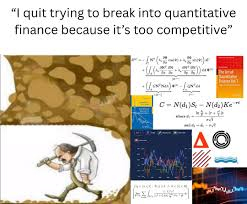
\includegraphics[width=1\linewidth]{dig.png}
\end{center}

\end{multicols*}

\begin{center}
    
\includegraphics[width=1\linewidth]{hft.png}
\end{center}

\end{document}